\section{Motion Selection based on Human Signs}
\label{sec:aural}
We construct a rule-based reaction system for a human user to activate the robot action. Preparing some sets of keyword and associated robot motion, the human can make the robot move with considering what action he/she wants the robot to take and how it can be realized combining the prepared rule-based actions. Although which order the robot moves completely relies on which order the human commands, this system sufficiently works in a household environment where the human wants the robot to be an obedient assistant. \tabref{speech_command} below shows the list of the prepared keywords and associated robot motions. For speech recognition, we use the system produced in our laboratory that is now published as an application for an android phone~\cite{ros_voice_message}.

\begin{table}[htbp]
  \begin{center}
    \caption{Speech commands.}
    \begin{tabular}{|l|l|l|} \hline
      usage & command & detail \\ \hline\hline
      Selection & Walk & walking mode \\
      of mode & Move arms & manipulating mode \\ \hline
      & Go forward & translate forward \\
      & Go back & translate backward \\
      & Go right & translate right\\
      Direction & Go left & translate left\\
      of walking & Turn right & rotate clockwise \\
      & Turn left & rotate counterclockwise \\
      & Come here & move in front of human \\
      & Go away & move opposite back \\ \hline
      Hand & Grasp (right/left) & grasp (right/left) hand \\
      motion & Release (right/left) & release (right/left) hand \\ \hline
      & Start & start motion \\
      Begin/End & Stop & stop motion \\
      & OK & completion of motion \\ \hline
      %% yes/no & ok & yes \\
      %% & no & no \\ \hline
      Selection & (right/left/both) shoulder & move (right/left/both) shoulder\\
      of limb & (right/left) elbow & move (right/left) elbow\\
      & (right/left) wrist & move (right/left) wrist\\ \hline
    \end{tabular}
    \label{table:speech_command}
  \end{center}
\end{table}

\begin{figure}[htbp]
  \begin{center}
    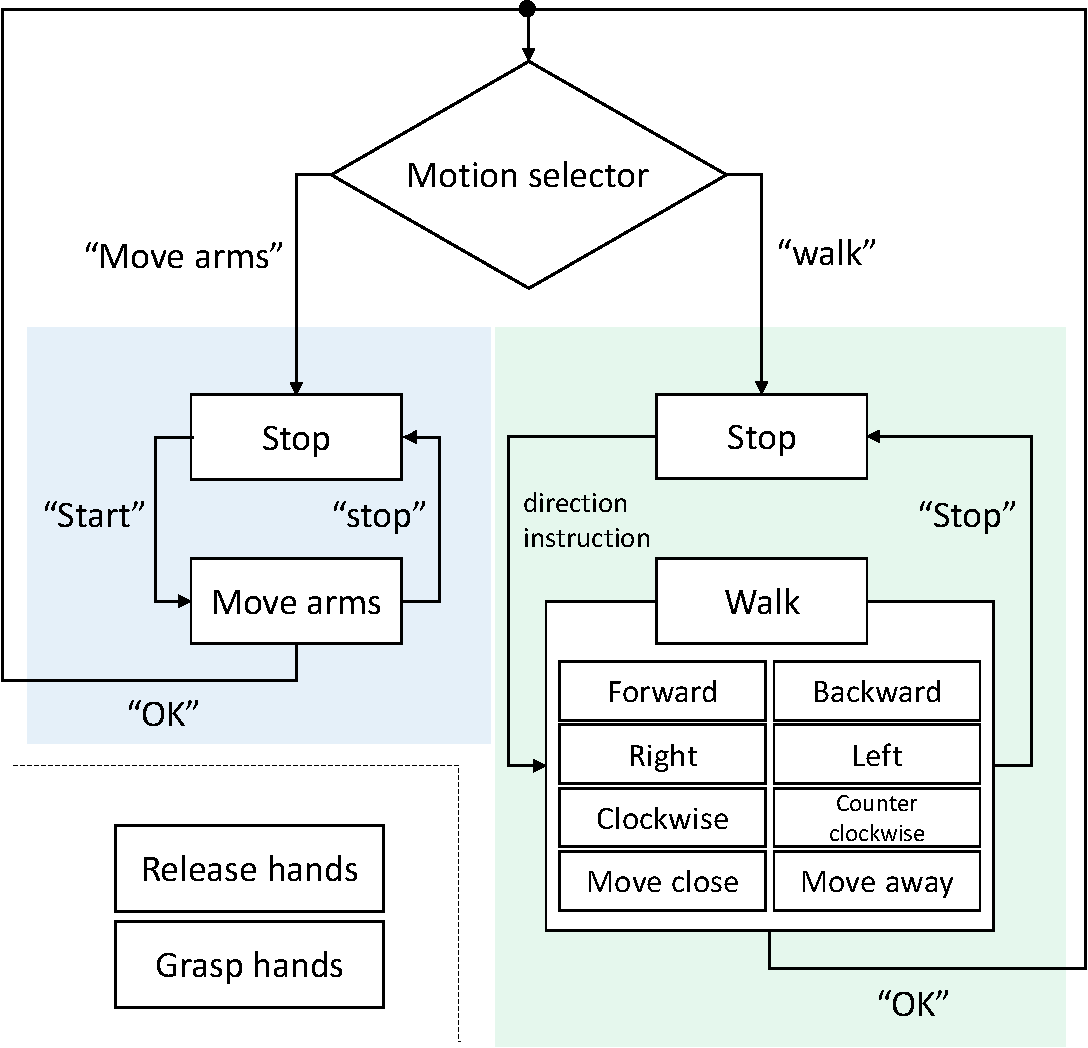
\includegraphics[width=0.80\columnwidth]{figs/motion_selector3}
    \caption{The state flow to execute several cooperative works. The states colored blue are the motions explained in \subsecref{move_hand}, and the the states colored green are the motions described in \subsecref{walk}. Lining up these motions parallelly with using aural interactions, continuous task execution can be realized.}
    \label{figure:speech_flow}
  \end{center}
\end{figure}

Using these rule-based commands, we combine the robot manipulating motions described in \subsecref{move_hand} and the walking motions described in \subsecref{walk} in parallel and enable them to be activated repeatably as shown in \figref{speech_flow}.

Added to these aural instruction commands, we attempt to induce robot movements not only by voice but also by other factors; force information and human standing position. Although the voice commands ensure the absolutely correct motion with the robot, considering human-human interaction, there must be other communication means during the cooperative works. For that kind of communication between a human and a robot, we introduce two characteristics to the robot in cooperative carrying. One is that when the robot feels strong force while the robot is not walking, the robot regards it as the suggestion to move in that direction where the force works. Another is that when the human moves sideward exceeding the threshold, the robot regards it as the sign to move sideward in that direction and starts to move. Note that using the motion described in \subsecref{walk}, there don't have to be excess internal force during carrying. These characteristics are only for the triggers of the walking motions.

\begin{figure}[htbp]
  \begin{center}
    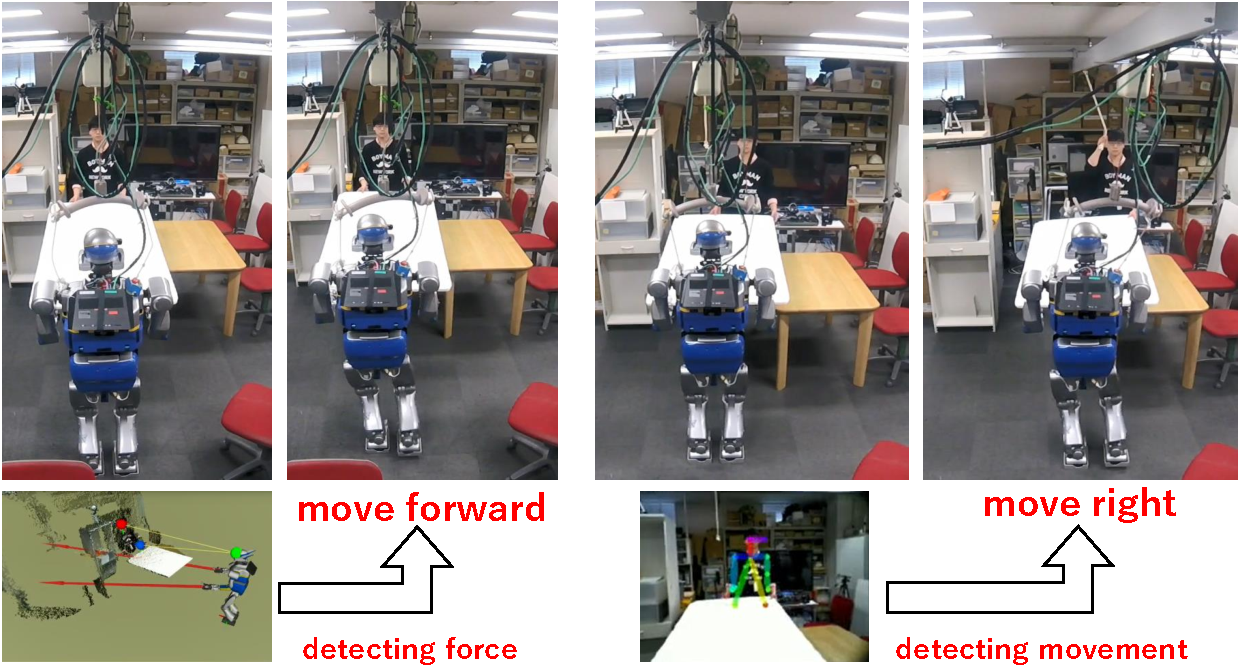
\includegraphics[width=1.00\columnwidth]{figs/transition}
    \caption{The examples of multimodal signs inducing the robot to start moving. The left represents the robot starting walking forward due to the force felt through the object. The right represents the robot starting walking to the right due to the human position.}
    \label{figure:transition}
  \end{center}
\end{figure}
